\documentclass[a4paper,11pt,twopage,numbers=noenddot]{scrbook}

\usepackage[top=2cm,lmargin=1in,rmargin=1in,bottom=3cm,hmarginratio=1:1]{geometry}
\usepackage[utf8]{inputenc}
\usepackage[english]{babel}
\usepackage{amssymb}
\usepackage{amsthm}
\usepackage{thmtools}
\usepackage{fancyvrb}
\usepackage{mathtools}
\usepackage{amsmath}
\usepackage{ifthen}
\usepackage{xspace}
\usepackage{hyperref}
\usepackage{makeidx}
\usepackage{graphicx}
\usepackage{listings}
%\usepackage[right]{showlabels}
%\usepackage[justific=raggedright,totoc]{idxlayout}

\addto\extrasenglish{%
  \renewcommand{\chapterautorefname}{Section}
  \renewcommand{\sectionautorefname}{Section}
  \renewcommand{\subsectionautorefname}{Subsection}
  }

\newcommand\chap[1]{%
  \chapter*{#1}%
  \chaptermark{#1}%
  \addcontentsline{toc}{chapter}{#1}}

\declaretheorem[name=Definition,style=definition,numberwithin=chapter]{definition}
\declaretheorem[name=Example,style=definition,sibling=definition]{example}
\declaretheorem[style=definition,numbered=no]{exercise}
\declaretheorem[name=Remark,style=definition,sibling=definition]{remark}
\declaretheorem[name=Assumption,style=definition,sibling=definition]{assumption}
\declaretheorem[name=Observation,style=definition,sibling=definition]{observation}
\declaretheorem[name=Theorem,sibling=definition]{theorem}
\declaretheorem[sibling=definition]{corollary}
\declaretheorem[name=Fact,sibling=definition]{fact}
\declaretheorem[sibling=definition]{lemma}
\declaretheorem[sibling=lemma]{proposition}

%%%%%%%%%%%%%%%%%%%%%%%%%%%%%%%%%%%%%%%%%%%%%%%%%%%%%%%%%%%%%%%%%%%%%%%%%%%
%                                                                         %
%                   Spacing settings                                      %
%                                                                         %
%%%%%%%%%%%%%%%%%%%%%%%%%%%%%%%%%%%%%%%%%%%%%%%%%%%%%%%%%%%%%%%%%%%%%%%%%%%
\setlength{\parindent}{0pt}
\setlength{\parskip}{6pt}
\setlength{\marginparsep}{0cm}

\title{Interactive web interface for the Loop/While interpreter}

\author{Johannes Kern}

\makeatletter
\hypersetup{
  pdftex,
  pdfauthor={\@author},
  pdftitle={\@title},
  % kill those ugly red rectangles around links
  hidelinks,
}
\makeatother

\usepackage{newunicodechar}
\newunicodechar{∀}{\ensuremath{\forall}}
\newunicodechar{∃}{\ensuremath{\exists}}
\newunicodechar{×}{\ensuremath{\times}}
\newunicodechar{ø}{\ensuremath{\emptyset}}
\newunicodechar{≤}{\ensuremath{\le}}
\newunicodechar{∈}{\ensuremath{\in}}
\newunicodechar{→}{\ensuremath{\to}}
\newunicodechar{⊆}{\ensuremath{\subseteq}}
\newunicodechar{⊗}{\ensuremath{\otimes}}
\newunicodechar{∧}{\ensuremath{\wedge}}


\usepackage{tikz}
\usetikzlibrary[topaths,positioning,calc,arrows,automata,cd]

\usepackage{float} %enables float option 'H' for figure etc.

\usepackage{pifont,mdframed}
\newenvironment{warning}
  {\par\begin{mdframed}[linewidth=2pt,linecolor=red]%
    \begin{list}{}{\leftmargin=1cm
                   \labelwidth=\leftmargin}\item[\Large\ding{43}]}
  {\end{list}\end{mdframed}\par}

\bibliographystyle{alpha}
\begin{document}
\pagestyle{plain}
\begin{titlepage}
\newcommand{\drop}{0.07\textheight}
\begin{center}
\begingroup%
\vfill
{\LARGE\textsc{%
Friedrich-Alexander-Universität\\[2mm]
Erlangen-Nürnberg%
}}\\[\drop]
{%
% trim= left bottom right top

\includegraphics[height=1.8cm,trim=0cm 0mm 0 0mm]{img/tcs}\\
\textsc{\large Chair for Computer Science 8}\\
\textsc{\large Theoretical Computer Science}}%\\[\drop]
\vfill
\rule{\textwidth}{1pt}\par
\vspace{0.5\baselineskip}
{% maybe \itshape?
  \Huge\bfseries
  \makeatletter
  \@title \\[1cm]
  \makeatother
\large\bfseries
Documentation and installation manual
}\\[0.5\baselineskip]
\rule{\textwidth}{1pt}\par
\vfill
{\Large{\makeatletter\@author\makeatother}
  %\\ {\large\normalsize{maybe-ur-mail@example.org}}
}
\vfill
% trim= left bottom right top

\includegraphics[height=1.8cm,trim=0cm -5mm 0 0mm]{img/fau}
\vfill
{\large Erlangen, \today}
\endgroup
\end{center}
\end{titlepage}

% vim: tw=80 spell spelllang=en nocul
%
\tableofcontents
%\include{src/examples}
\chapter{Overview}
\section{Introduction}
In typical undergraduate courses in theoretical computer science, a major aspect is to discuss different models of computability and
their expressiveness. One important result is, that primitive recursion is not Turing complete, i.e. not equivalent to Turing machines or $\mu$-recursion.
In \cite{Hoffmann2018}, the difference in computational power between $\mu$-recursion and primitive-recursive computation is presented by
the languages WHILE and LOOP, where WHILE is a Turing-complete imperative language
that offers basic control constructs like while loops and if-then-else, and LOOP is a restriction of WHILE that allows only a restricted 
loop construct \textit{\textbf{loop} x \textbf{do} ... \textbf{enddo}}, which is to be understood as "execute ... as often as the value of x".

In preliminary work, an interpreter for a variation of this two languages was developed \cite{Gebhard2018}. Currently the only available IDE for
this languages is IntelliJ in combination with a plugin that is released together with the interpreter. The goal of this project was
to develop an web-based interactive interface to that interpreter such that no extra software has to be actually installed on the user's
computer. Additionally, the web interface provides an interactive tutorial which helps the user to learn the Loop/While language and
documents the usage of the web interface. 

\section{License information and used third-party software}
The software that was implemented as part of this project makes use of several CSS and javascript libraries that
have to be made available to the user for the web-application to work properly, so licensing issues have to be considered.

The frontend uses a publicly available CSS from the purecss project\footnote{https://purecss.io/} which 
is published under the Yahoo BSD license\footnote{https://github.com/pure-css/pure-site/blob/master/LICENSE.md}.

For user code inputs, the open source javascript-based BSD-licenced editor ace\footnote{https://ace.c9.io/} ist used.
Its code has been augmented by two source files (mode-LoopWhile.js and 
snippets/LoopWhile.js) to provide syntax highlighting for the Loop/While language. The new code must again be released under
the BSD License.

%To receive the input data for the program the interpreter is executing and 
%to display its output, we made use of the jQuery AJAX Terminal\footnote{https://github.com/n0nick/terminal}, which is published
%under GPL\footnote{https://www.gnu.org/licenses/gpl-3.0.txt}.

All these libraries can be redistributed under the same corresponding license terms.
The used copyrighted code mentioned above is also clearly separated from the code developed
in this project, and since the BSD license is copyleft free, the framework itself is not affected by obligations of those licenses.

On the server-side, a Python-based lexer library\footnote{https://gist.github.com/eliben/5797351} is used. A comment in the code
states that "This code is in the public domain", so there are no obligations with it.
Furthermore, we use the Python libraries TurboGears\footnote{https://www.turbogears.org/} and Autobahn\footnote{https://crossbar.io/autobahn/},
which are licensed under MIT license, and genshi\footnote{https://genshi.edgewall.org/}, which is licensed
under a BSD license. Since all there libraries are linked dynamically, the Python source code of the backend has no obligations to be
published under some certain license.

To execute the Loop/While code itself, the Interpreter of Michael Gebhard is used\cite{Gebhard2018}. Its code is licensed under the terms
of the Apache license\footnote{http://www.apache.org/licenses/LICENSE-2.0}, but not published yet. For this project, the code has been modified such that
error messages do not spoil paths or other sensitive information to the user. The Interpreter itself is not linked again the web interface,
but is used as a command-line tool.
Therefore, the code of the backend is not affected by obligations of that license. The modified interpreter code does not need to be published,
unless the interpreter binary itself is made available publicly.

\section{Software architecture}
The main part of the software that was developed in this project is written in Python 3 and relies on the web 
framework TurboGears in combination with the XML-template engine genshi.

It uses the widely-used model-view-controller (MVC) pattern \cite{Starke2011} to separate view-related concerns from
internal processes like the connection to the interpreter/debugger.


\begin{figure}[H]
    \centering
    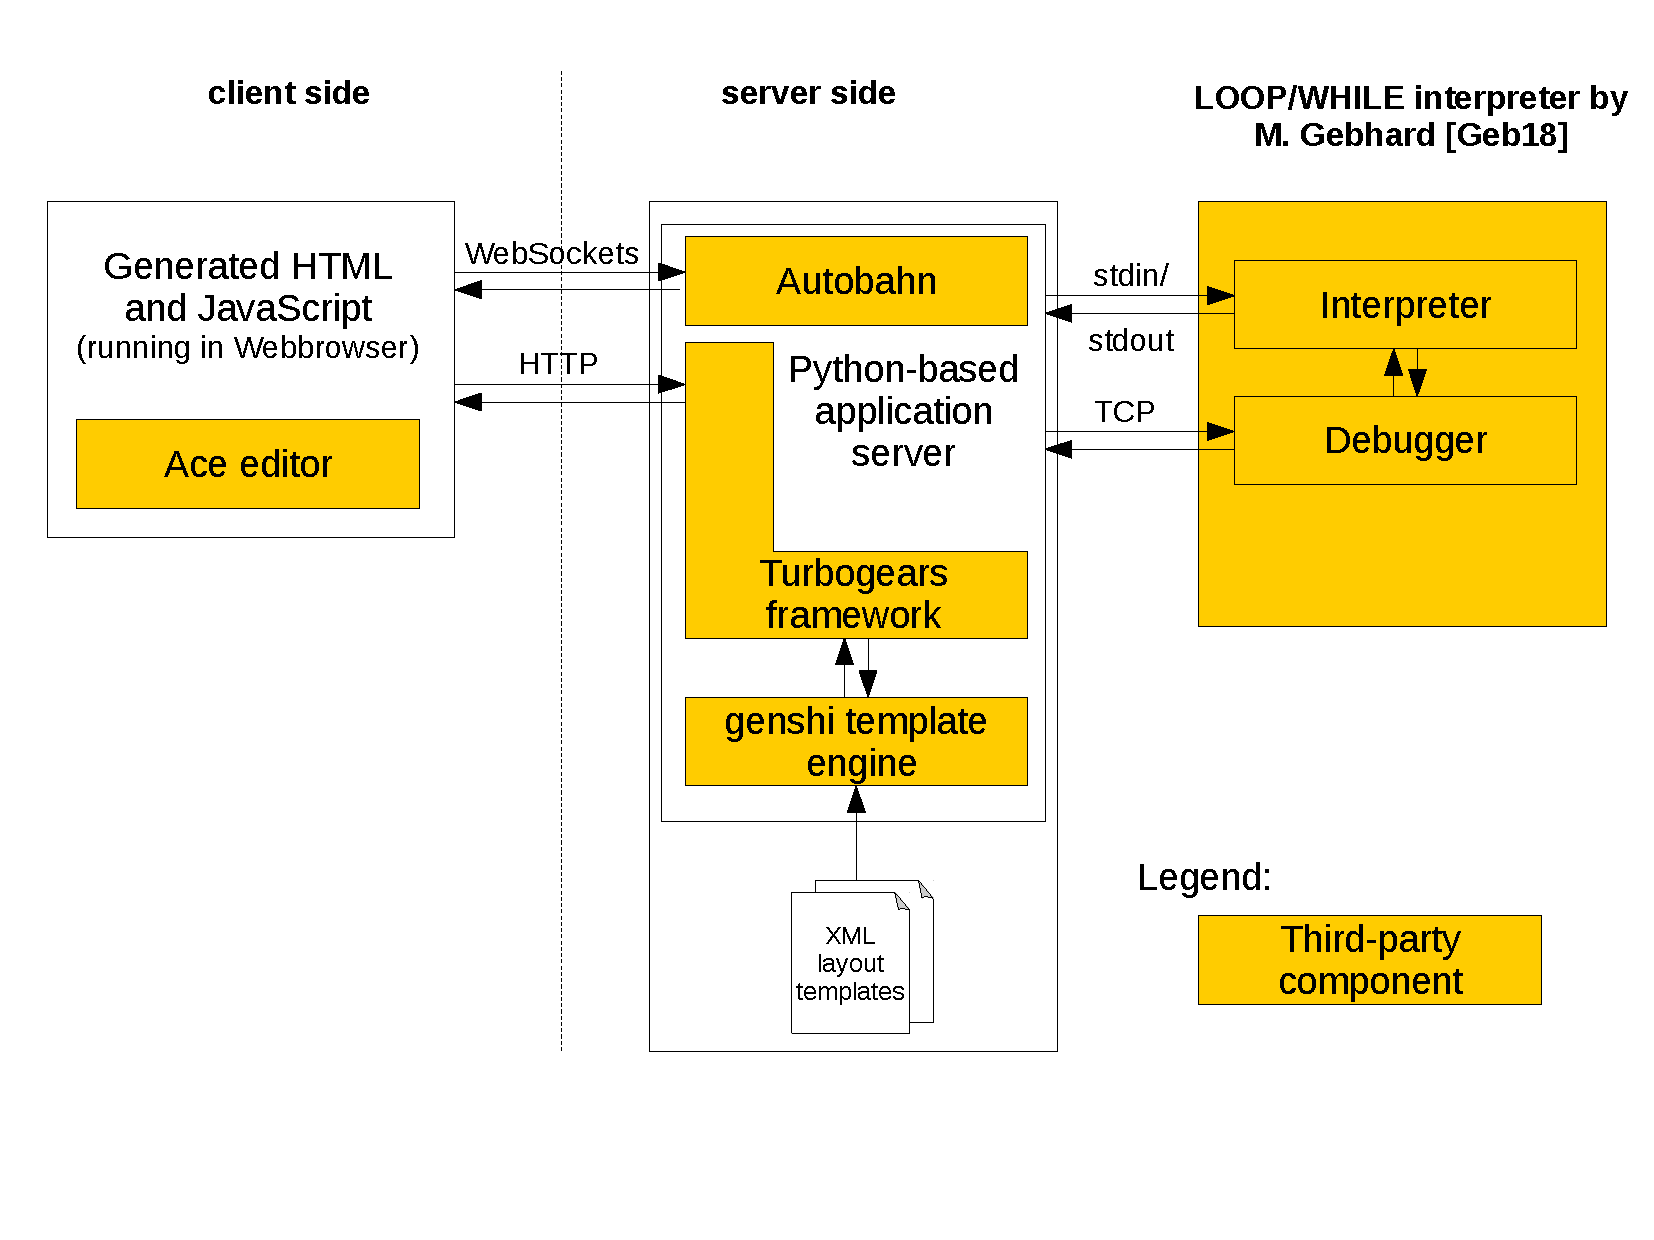
\includegraphics[width=340px]{img/Architecture.pdf}
    \caption[Software architecture]{Software architecture}
    \label{fig:software_arch}
\end{figure}

The view on the client side has two different modes: the interpreter and the debugger mode.
In the interpreter mode, the user sees an editor, realized
by the Ace editor library, in which he can edit his code. When the user clicks the run button, the JavaScript in the browser sends a
request to the server, containing the user's program, and the server replies a randomly generated session id. This session id is then
used by the script for authentication in further requests, e.g. when the contents of the terminal are updated or an user input is transmitted
to the server. On the server side, a child process running the lwre binary is spawned to run the user's Loop/While code. The session (and therefore 
also the child process) is terminated, when either 1) the program terminates itself, 2) the user clicks the stop button or 3) a timeout elapses.

When the user clicks the debug button, the view switches to the debug mode, and the editor is replaced by a HTML-table containing the content of
the editor, with the ability to display breakpoints and highlighting of the currently executed line, as it is needed by the debugger. This view is
generated on the server side and also the child process is spawned when entering the debug mode, since the connection to it is not only necessary
when the program runs, but also to set breakpoints before the execution of the user's code is started.

\section{Communication protocols}
The communication between the client JavaScript and the Python-based server relies on two different OSI Layer 7 protocols.

The first one used for synchronous communication is based on HTTP. It provides several commands to start and stop sessions, transmit user
input in the terminal and to set breakpoints:

\begin{tabular}{l l l}
\hline
relative URL           & POST arguments      & server response\\
\hline
run                    & program\textunderscore code        & \textless SESSION\textunderscore ID\textgreater\space in case of success, 0 in case\\
                       &                                    & of error\\
stop                   & session\textunderscore id          & "OK" in case of success, \textless ERR\textunderscore MSG\textgreater\space in case\\
                       &                                    & of error\\
shell                  & input, session\textunderscore id   & \textless STRING\textgreater\space to print on the terminal\\
check\textunderscore termination\text{*}        & session\textunderscore id          & "running", "terminated", "timeout" or "error"\\
start\textunderscore debug\textunderscore session    & program\textunderscore code        & "OK," + \textless SESSION\textunderscore ID\textgreater\space in case of success,\\
                       &                                    &  "FAIL," + \textless ERR\textunderscore MSG\textgreater\space otherwise\\
debugger               & session\textunderscore id          & an HTML \textless div\textgreater\space -tag containing the\\
                       &                                    & debugger view\\
set\textunderscore breakpoint         & session\textunderscore id, line\textunderscore no & "OK" or "FAIL"\\
remove\textunderscore breakpoint      & session\textunderscore id, line\textunderscore no & "OK" or "FAIL"\\
debugger\textunderscore poll\textunderscore state\text{*}   & session\textunderscore id, line\textunderscore no & "DIED", "RESTARTED", "FAIL" or a JSON-\\
                       &                                    & string containing the last stacktrace\\
debugger\textunderscore action        & session\textunderscore id, action\text{**}     & "OK" or "FAIL"\\
\hline
\end{tabular}

\text{*} deprecated commands that were used before the WebSockets-based protocol was developed.\\
\text{**} the following actions are available:

\begin{tabular}{l l l}
\hline
action      & describtion \\
\hline
start       & starts the debugger and stops at the first line of the root macro\\
continue    & continues the debugger until the next breakpoint is reached.\\
stepinto    & steps to the next line\\
stepover    & steps to the next line without entering macros\\
stepout     & steps out of the current macro\\
close       & stops the debugger and closes the session. The session id gets invalidated\\
\hline
\end{tabular}

For asynchronous communication, another protocol based on HTML5 WebSockets is used.
When a client has started the interpreter or debugger, it connects to the WebSockets
server and transmitts its session id for authentification. By this communication channel,
the client gets notified when the status of the lwre changes, a line can be printed on the
terminal or a debugger breakpoint is reached.

\section{Repository structure}
\begin{tabular}{l l}
\verb|src/|           & source for the backend\\
\verb|templates/|     & XML/XHTML templates for turbogears\\
\verb|web/|           & files that will be directly served by the web server\\
\verb|unit_tests/|    & unit tests for the backend\\
\verb|test_programs/| & test programs that are used by the unit tests\\
\verb|config/|        & sample configuration files
\end{tabular}

\chapter{Local Installation and configuration}
\label{chapter:installation}
\begin{warning}
Recommendation: Instead of local installation, a Docker container should be used (see \autoref{chapter:docker}).
\end{warning}

\section{Requirements}
We assume, that there is a Linux-based system (e.g. Ubuntu or Debian) with at least Python 3.5 installed. TurboGears and other prerequisites can
be installed by the package-management system of Python (depending on your installation, you might need the command pip3 instead of pip for Python 3):

\begin{verbatim}
pip install TurboGears2 genshi transaction waitress autobahn[twisted,accelerate]
\end{verbatim}

This manual expects also an installed nginx web server, but usage of other web servers like Apache httpd\footnote{https://httpd.apache.org/}
should be possible without problems.

The Loop/While Interpreter binary is expected to be compiled separately from the branch
\mbox{'webinterface'} of the repository\\
%\url{https://git8.cs.fau.de/theses/michael-gebhard-ba/loopwhile-yacc-interpreter}.
\url{https://git8.cs.fau.de/software/loopwhile-yacc-interpreter}.


\section{Installation}
\label{section:installation}
There is a script \verb|deliver.sh| in the repository, that does most of the necessary
steps automatically. The variables used in this script can be adjusted:

\begin{tabular}{@{}l l}
\verb|USER|, \verb|GROUP| & the user- and group name that gets owner of the installation directories\\
                          & and which are running the daemon \\
\verb|INSTALL_DIR|        & directory in which the Python-based backend will be installed \\
\verb|USER_SRC_DIR|       & directory used to create temporary files. This directory must be exclusively\\
                          & used by the backend \\
\verb|HTTPD_DIR|          & directory to which all files are copied that will be directly served by nginx\\
                          & or Apache httpd\\
\end{tabular}

After this script is executed, all necessary files are placed to their correct location.

The next step is to set up the web server. An example configuration for nginx can be found
in the repository under \verb|config/nginx.example|. This file must be copied to\\ \verb|/etc/nginx/sites_available|,
and a symlink to this copy must be placed under\\ \verb|/etc/nginx/sites_enabled|. In this configuration, requests to
the HTTP backend are delegated to the port 8080 and requests to the WebSockets backend get delegated to port 8081.
Furthermore, the configuration ensures, that the original client IP address is transmitted in the request header to
the respective backend to enable further request filtering there.

The last step is to set up a daemon for the backend. An example configuration file for systemd is found in the
repository under \verb|config/lw.service|. This file must be copied to \verb|/etc/systemd/system/lw.service|
and the settings for \verb|User|, \verb|ExecStart| and \verb|WorkingDirectory| have to be adjusted.
The daemon can then be started by
\begin{verbatim}
sudo systemctl start lw
\end{verbatim}
To start the service automatically on boot, you have to enable it:
\begin{verbatim}
sudo systemctl enable lw
\end{verbatim}

\section{Configuration and run script}
\subsection{Overview}
\label{section:config}
The entry point of the backend daemon in the \verb|run.sh| script. In this script, some basic
parameters can be set:

\begin{tabular}{@{}l l}
\verb|--logile=<PATH>|                          & Path to the logfile that shall be generated.\\
                                                             & A RotatingFileLogger is used.\\
\verb|--loglevel=<LEVEL>|                       & Level used for logging. The higher the level, the more\\
                                                             & verbose the logging.\\
                                                             & Available levels are: CRITICAL, ERROR, WARNING,\\
                                                             & INFO, DEBUG, NOTSET. Default is INFO.\\
\verb|--host=<HOST_ADDR>|        & Address on which the backend listens on. It is strongly\\
                                                             & recommended to use 127.0.0.1 here, so that the backend\\
                                                             &  itself is only reachable by the upstream web server.\\
\verb|--port=<PORT>|                           & Port the backend listens on\\
\verb|--user_src=<PATH>|         & Path to the directory for temporary files\\
\verb|--max_sessions=<LIMIT>|  & Maximal number of sessions, i.e. concurrent instances\\
                                                             & of the lwre binary\\
\verb|--ws_interface=<URL>|      & Address on which the WebSockets service listens on.\\
                                                             & It is strongly recommended to use 127.0.0.1 here.\\
\verb|--ws_post=<URL>|           & Port the WebSockets service listens on\\
\verb|--report_file=<PATH>|           & File to which report data will be written\\
\verb|--max_sessions_per_addr=<LIMIT>|           & Maximal number of sessions per IP address\\
\end{tabular}

For testing purposes, the \verb|run.sh| script can also be executed directly without running the install routines.

\subsection{Security and performance}
The nginx settings in \verb|config/| do not use HTTPS at all. However, it is strongly recognized
to set up the server such that it is only reachable by HTTPS.

Performance tests on a virtual server with 2 virtual CPUs and 2GB of RAM showed, that the application is able to handle over 128 parallel debugging
sessions without recognizable impact to the response times. Nevertheless, the maximal number of parallel sessions is
limited by
\begin{itemize}
    \item the maximal number of processes allowed by the operating system
    \item the maximal number of open files in the server process
    \item the limit configured using the \verb|--max_sessions| option (see Section \ref{section:config}).
\end{itemize}

The limits of the operating system can be obtained by the shell command \verb|ulimit -a|.
For the lw server daemon, they can be adjusted if necessary by adding the following two lines
in the systemd service file (\verb|/etc/systemd/system/lw.service|):
\begin{verbatim}
[Service]
...
LimitNOFILE=20000
LimitNOFILESoft=20000
LimitNPROC=20000
LimitNPROCSoft=20000
\end{verbatim}

To reduce the risk of (distributed) DoS attacks, it is
possible to establish a limit of parallel sessions per IP address, using the \verb|--max_sessions_per_address| option.
To determine a suitable limit, the report generator is a useful tool (see Section \ref{section:reportgen}).

Another way is to restrict the maximal number of TCP connections per time unit in the firewall (using iptables).

\subsection{Report generator}
\label{section:reportgen}
The report generator can be used to generate certain usage statistics. It writes status data at runtime to a
file that is specified by the \verb|--report_file| argument. The data contained in this file is persistent
even after restarts of the server daemon.

To generate statistics, you have to call the respective Python script:
\begin{verbatim}
python3 src/ReportGenerator.py --infile=<PATH>
\end{verbatim}
This script uses different metrics and can easily be extended.


\section{Tutorial generator}
The tutorial is generated using an own simple markup language, that provides some basic features
for text formatting and syntax highlighting for code snippets. A tutorial template according
to this markup language is a sequence of text and commands described in the following table.
Commands start with a backslash and cannot be nested. To be used in text, the backslash is escaped
by double backslash.

\begin{tabular}{@{}l | l}
\textit{\textbackslash headline \{ \textless text\textgreater\space \} } & headline of the tutorial\\
\textit{\textbackslash tableofcontents} & a table of contents which is generated\\
                         & automatically\\
\textit{\textbackslash code \{ \textless code\textgreater\space \} } & syntax highlighted view of a given\\
                                                & LOOP/WHILE code\\
\textit{\textbackslash html \{ \textless text\textgreater\space \} } & HTML code that gets directly embedded\\
        \begin{tabular}{@{}l l}
        \textit{\textbackslash link} &\{ \textless target\textunderscore url\textgreater\space \}\\
                      &\{ \textless link\textunderscore text\textgreater\space \}
        \end{tabular} 
       &\begin{tabular}{@{}l}
        a link to \textless target\textunderscore url\textgreater\space\\\space\\
        \end{tabular}\\
\textit{\textbackslash nobr \{ \textless text\textgreater\space \} } & A piece of text that should not contain a line break
\end{tabular}

The other commands are self-explanatory:\\
\textit{\textbackslash chapter \{ \textless text\textgreater\space \} },
\textit{\textbackslash section \{ \textless text\textgreater\space \} },\\
\textit{\textbackslash bold \{ \textless text\textgreater\space \} },
\textit{\textbackslash italic \{ \textless text\textgreater\space \} },
\textit{\textbackslash linebreak}

The Tutorial Generator is started by just running the corresponding Python
source file, specifying input and output file on the command line:
\begin{verbatim} 
python3 src/TutorialGenerator.py --infile=<TEMPLATE_FILE> --outfile=<OUTPUT_PATH>
\end{verbatim}
This script is usually executed automatically by the \verb|deliver.sh| script
described in section~\ref{section:installation}, expecting the tutorial template in
\verb|templates/tutorial.template|. It will place the output in 
\verb|templates/tutorial_container.xml|.
%\newpage
Example:
\lstset{basicstyle=\footnotesize}
\begin{lstlisting}[frame=single]
\headline{Headline of the Tutorial}
\tableofcontents
\chapter{example chapter}
  \section{example section}
    This is normal text.
    \bold{This is bold text.}
    \italic{This is italic text.}
    \linebreak
    \link{http://example.com}{This is a link.}
    \code{
//This is a Loop/While code snippet
in: i0
out: o0

o0 := i0
    }
\end{lstlisting}

\chapter{Docker container}
\label{chapter:docker}
This chapter describes how the loopwhile interactive interpreter service
is installed using a Docker container. The container bundles the application
together with an up-to-date nginx which is fully preconfigured.


\section{Installation}
The only requirement is an installation of Docker itself.
The application is installed in three steps:
\begin{itemize}
\item Clone the git repository of the interactive interpreter to the machine
      on which the service shall run
\item Run \verb|./build_container.sh| to build the container
\item Run \verb|./run_container.sh| to start the container. The service is then
      listening on port 80
\end{itemize}



\section{Logfiles}
In the directory that contains the \verb|./run_container.sh| script, a subdirectory
\verb|logs| will be created, which is used to store all relevant logfiles. There
you will find one subdirectory for each service:
\begin{itemize}
\item \verb|loopwhile|: Logfiles of the lw service
\item \verb|nginx|: Logfiles of nginx
\item \verb|supervisor|: Logfiles of the supervisord deamon. Additionally,
      stderr and stdout of all supervised services are captured.
\end{itemize}

\bibliography{literature}
\end{document}

% vim: tw=80 nospell spelllang=en nocul
